\subsection{Assessing of Ignorance} \label{ut-fail}

Initially we've declared importance of having tests and ecosystem for their automation but there were not written any 
valuable amount of them (10\% coverage, \ref{a-badges}). That was done to show a consequence of such a decision -- not 
to write tests. So, let's measure made mistakes during our Increment (four Iterations, two weeks each):

\begin{lstlisting}[language=bash]
git log --format="%ad %s" --grep="\[BF\]" --date=iso | \
awk -F ' ' '{print $1}' | \
sort | \
uniq -c
\end{lstlisting}

\noindent \q{git log}-command retrieves a commit history (\q{\%ad} - to include the commit date, \q{--date=iso}-option 
converts dates to ISO 8601 [YYYY-mm-dd]; \q{\%s} - take subject) with the specified format via \q{--grep} (since we've 
used \q{[BF]}-prefix in a title for created bug-reports [issues] and used it as a part of the commit message). \q{awk} 
extracts the date part from each line and delegate sorting to \q{sort}-command by the extracted dates. Finally, 
\q{uniq -c}-command counts the occurrences of each unique date. And the same operation we'll do for the \q{fix}-keyword.

\begin{figure}[h]
  \begin{center}
    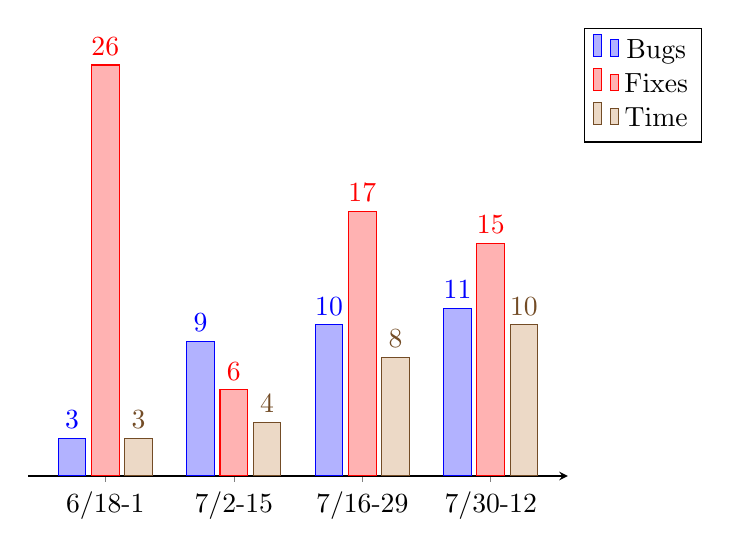
\begin{tikzpicture}
      \begin{axis}[ybar, symbolic x coords={6/18-1, 7/2-15, 7/16-29, 7/30-12},
        legend pos=outer north east, axis y line=none, axis x line=bottom, nodes near coords, enlarge x limits=0.2, ] 
      \addplot+ coordinates {(6/18-1, 3) (7/2-15, 9) (7/16-29, 10) (7/30-12, 11)}; 
      \addplot+ coordinates {(6/18-1, 26) (7/2-15, 6) (7/16-29, 17) (7/30-12, 15)}; 
      \addplot+ coordinates {(6/18-1, 3) (7/2-15, 4) (7/16-29, 8) (7/30-12, 10)}; 
      \legend{Bugs, Fixes, Time}; \end{axis} 
    \end{tikzpicture} 
  \end{center}
  \caption{Counting made mistakes per each Iteration}\label{im-errors}
\end{figure}

\noindent \q{Time} -- how many hours was spent to fix identified issues (where 28 hours - allocated time per Iteration);
\q{Bug} and \q{Fixes} -- counters, retrieved from our git history.\\
\\

Current project was spearheaded by a lone developer, while additional team members could potentially increase 
the needed efforts \cite{Alm21} to maintain the application stability. Returning back to our chart, it shows us 
that up to a third of the allotted time was spent on fixing bugs -- by adhering to the principle of zero 
defects distribution \cite{Allan98}. In the business realm, companies sometimes opt to overlook issues and instabilities 
while augmenting functional capabilities through the introduction of new features. This can inadvertently create a ticking 
time bomb, culminating in substantial financial and reputational losses. That's why the cost to brand perception is 
frequently greater than the cost of finding and fixing a bug during development. By example, National Institute of 
Standards and Technology found that software bugs cost (in 2002) the US economy \$59.5 billion every year, and 
\$22.2 billion could be eliminated by improved testing \cite{RTI02}.

Simply saying, the consequence of missed tests is a broken managerial triangle: out from a scope, time, and budget.
Neither Agile transformation, nor micromanagement would help to be predictive in delivery. To mitigate potential adverse 
outcomes, a widely adopted strategy involves instigating a technical iteration, or designating a specific period, often 
at the close of a calendar year, for dedicated bug-related work. As a testament to robust processes, the fundamental 
principle of quality permeates all stages and serves as a cultural cornerstone. Non-functional requirements, serving 
as a tool to ensure quality throughout every phase, can find a practical application here \cite{Sam17}, \cite{Suz12}. 

Test-Driven Development approach is known from 1999 year as Extreme Programming flow, but for unknown to me reason 
not widely spread. Argumentation that "we do not have a time to write tests" is the same as "we won't use a car since 
already running to reach our 200km target within a day" (instead of a few hours). In Agile transformations it's a mantra 
that the usage of Scrum (communication framework) will increase development flow 10 times. By looking wider, 
Agile, DevOps, Lean, and other approaches put an emphasis on the quality throughout the process. It's so since a 
communication itself has a natural limitation in the achievable performance optimization. Next 10x boost can be reached 
by growing exceptionally a technical excellence. Observing developers dedicating half a day to test a seemingly 
"one-hour" change, we may find it perplexing that the idea of investing an additional hour in crafting tests is met with 
resistance.

As an example, by achieving the technical excellence through a semaphore approach ("red" - write test for the missed 
part of a code, assert expectations; "yellow" - write code to pass tests; "green" - refactor your code) the 
stabilization phase, "monthly" regression testing, even a separate QA Department won't be needed. All acceptance 
criteria for user story, feature, and even epic are transliterated into tests, and controlled by automation. That 
reinforces the developer's mental model of the code, boosts confidence and increases productivity.
